\documentclass[12pt, a4paper]{article}

\usepackage{balance}
\setlength{\columnsep}{1 \baselineskip}

\newenvironment{Figure}
  {\par\medskip\noindent\minipage{\linewidth}}
  {\endminipage\par\medskip}

\usepackage{caption}

\usepackage[utf8]{inputenc}
\usepackage[english]{babel}

\usepackage[font=small,labelfont=bf]{caption}

\usepackage{amsmath}

\interdisplaylinepenalty = 2500

\usepackage{mathtools}

\usepackage{amssymb}

%\usepackage{stmaryrd}

\usepackage{amsthm}

%\usepackage{latexsym}

\usepackage{IEEEtrantools}

\usepackage{eucal}

\usepackage{bbm}

\usepackage{scalerel}

\usepackage[dvipsnames]{xcolor}
\definecolor{darkgreen}{RGB}{35, 89, 52}
\definecolor{paleorange}{RGB}{255, 236, 207}
\definecolor{paleteal}{RGB}{223, 245, 243}
\definecolor{palered}{RGB}{255, 234, 232}

\usepackage{graphicx}
\graphicspath{ {./images/} }

\usepackage{tikz}
\usetikzlibrary{arrows}
\usepackage{tikz-cd}

\usepackage{hyperref}
\hypersetup{
	colorlinks=true,
	linkcolor=darkgreen,
	filecolor=magenta,      
	urlcolor=MidnightBlue,
	citecolor=darkgreen,
	pdftitle={Dynamic codesign in Poly},
	bookmarks=true
}


\usepackage[
backend=bibtex,
maxbibnames=50,
style=alphabetic,
citestyle=alphabetic]{biblatex}
\addbibresource{candoc.bib}
%Remove In: from journal articles
\renewbibmacro{in:}{%
  \ifentrytype{article}{}{\printtext{\bibstring{in}\intitlepunct}}}


\theoremstyle{definition}

\newtheorem{counter}{Definition}[section]

\newtheorem{definitionx}[counter]{Definition}
\newenvironment{definition}
  {\pushQED{\qed}\renewcommand{\qedsymbol}{$\triangleleft$}\definitionx}
  {\popQED\enddefinitionx}

\theoremstyle{plain} 
\newtheorem{lemma}[counter]{Lemma}

\theoremstyle{plain} 
\newtheorem{proposition}[counter]{Proposition}

\theoremstyle{plain}
\newtheorem{theorem}[counter]{Theorem}

\theoremstyle{plain}
\newtheorem{question}[counter]{Question}

\theoremstyle{plain}
\newtheorem{problem}[counter]{Problem}

\theoremstyle{remark}

\newtheorem{examplex}[counter]{Example}
\newenvironment{example}
  {\pushQED{\qed}\renewcommand{\qedsymbol}{$\diamond$}\examplex}
  {\popQED\endexamplex}

\newtheorem*{excont}{Example \continuation}
\newcommand{\continuation}{??}
\newenvironment{continueexample}[1]
{\renewcommand{\continuation}{\ref{#1}}\excont[continued]}
{\endexcont}

\theoremstyle{remark}
\newtheorem{remark}[counter]{Remark}

\usepackage[most]{tcolorbox}
\newtcbtheorem[number within=section]{tcdefinition}{Definition}{colback=paleteal,colframe=NavyBlue,fonttitle=\bfseries, breakable, enhanced}{def}

\newtcbtheorem[number within=section, use counter from = tcdefinition]{tctheorem}{Theorem}{colback=paleteal,colframe=NavyBlue,fonttitle=\bfseries, breakable, enhanced}{thm}

\newtcbtheorem[number within=section, use counter from = tcdefinition]{tcexample}{Example}{colback=paleorange,colframe=BurntOrange,fonttitle=\bfseries, breakable, enhanced}{ex}


\newtcbtheorem[number within=section, use counter from = tcdefinition]{tcremark}{Remark}{colback=white,colframe=gray,fonttitle=\bfseries, breakable, enhanced}{rem}

\newtcbtheorem[]{tcproblem}{Problem}{colback=palered,colframe=Bittersweet,fonttitle=\bfseries, breakable, enhanced}{pr}

\newcommand{\zuz}[1]{%
	
	\begin{tikzpicture}[#1]%
	
	\draw[semithick, line cap = round, line join = round] (-0.3ex,0.35ex) -- (0.5ex,0.35ex);
	
	\draw[semithick, line cap = round, line join = round] (0.5ex,0.35ex) -- (0.5ex,-0.5ex);
	
	\draw[semithick, line cap = round, line join = round] (0.5ex,-0.5ex) -- (1.5ex,-0.5ex);
	
	\draw[semithick, line cap = round, line join = round] (0,0) -- (1ex,0);%
	
	\draw[semithick, line cap = round, line join = round] (1ex,0) -- (1ex,-0.85ex);
	
	\draw[semithick, line cap = round, line join = round] (1ex,-0.85ex) -- (1.8ex,-0.85ex);
	
	\end{tikzpicture}%
	
} 

\renewcommand\qedsymbol{\zuz{scale=1.5}}

\newcommand{\mc}[1]{\mathcal{#1}}

\newcommand{\sub}{\subseteq}

\newcommand{\upper}{\mathsf{U}}
\newcommand{\upc}[1]{\uparrow{#1}}

\newcommand{\low}{\mathsf{L}}
\newcommand{\lwc}[1]{\downarrow{#1}}

\newcommand{\op}[1]{#1^{\text{op}}}

\newcommand{\slens}[2]{\raisebox{0.4ex}{\scaleobj{0.25}{\begin{pmatrix} \scaleobj{3}{{#1}} \\ \scaleobj{3}{{#2}} \end{pmatrix}}}}
\newcommand{\lens}[2]{\scaleobj{0.6}{\begin{pmatrix} \scaleobj{1.3}{{#1}} \\ \scaleobj{1.3}{{#2}} \end{pmatrix}}}
\newcommand{\blens}[2]{\scaleobj{0.9}{\begin{pmatrix} {#1} \\ {#2} \end{pmatrix}}}

\makeatletter
\def\slashedarrowfill@#1#2#3#4#5{%
	$\m@th\thickmuskip0mu\medmuskip\thickmuskip\thinmuskip\thickmuskip
	\relax#5#1\mkern-7mu%
	\cleaders\hbox{$#5\mkern-2mu#2\mkern-2mu$}\hfill
	\mathclap{#3}\mathclap{#2}%
	\cleaders\hbox{$#5\mkern-2mu#2\mkern-2mu$}\hfill
	\mkern-7mu#4$%
}
\def\rightslashedarrowfill@{%
	\slashedarrowfill@\relbar\relbar\mapstochar\rightarrow}
\newcommand\xslashedrightarrow[2][]{%
	\ext@arrow 0055{\rightslashedarrowfill@}{#1}{#2}}

\def\leftslashedarrowfill@{%
	\slashedarrowfill@\relbar\relbar\mapstochar\leftarrow}
\newcommand\xslashedleftarrow[2][]{%
	\ext@arrow 0055{\leftslashedarrowfill@}{#1}{#2}}
\makeatother

\newcommand{\prof}{\xslashedrightarrow{}}
\newcommand{\bprof}{\xslashedleftarrow{}}

\title{Dynamic codesign in \textsf{Poly}}
\author{Marius Furter}


\begin{document}

\maketitle
\tableofcontents

\section{Recap of \textsf{Poly}}
Recall that a \emph{representable functor} has the form $\mathcal{C}(A,-) : \mathcal{C} \rightarrow \mathsf{Set} $. When $\mathcal{C} = \mathsf{Set}$, we will denote $\mathsf{Set}(A,-) =: y^A$ and call this a \emph{monomial}. A \emph{polynomial functor} is any functor that is isomorphic to a sum of monomials
$$p \cong \sum_{i \in I} y^{p[i]},$$
where the $(p[i])_{i \in I}$ is a family of sets, and the sum is taken to be the coproduct in the functor category $[\mathsf{Set},\mathsf{Set}]$ given by taking the component-wise disjoint union of the sets in question. Observe that if we evaluate $p$ at the singleton set $1$, we recover the indexing set of the sum
$$p(1) \cong \sum_{i \in I} 1^{p[i]} \cong \sum_{i \in I} 1 \cong I.$$
Hence we will often write $p \cong \sum_{i \in p(1)} y^{p[i]}$ to avoid always having to name the index set. The elements of $p(1)$ are called the \emph{positions} of $p$, while the elements of $p[i]$ are called the \emph{directions} at position $i$.

Since polynomial functors are functors, morphisms between them are given by natural transformations. By using the universal property of coproducts in $[\mathsf{Set},\mathsf{Set}]$ along with the Yoneda lemma, one can observe that
\begin{IEEEeqnarray*}{rCl}
	\mathsf{Poly}(p,q) &=& \mathsf{Poly}(\sum_{i \in p(1)} y^{p[i]},\sum_{j \in q(1)} y^{q[j]}) \\
	&\cong& \prod_{i \in p(1)} \mathsf{Poly}(y^{p[i]},\sum_{j \in q(1)} y^{q[j]}) \\
	&\cong& \prod_{i \in p(1)} \sum_{j \in q(1)} {p[i]}^{q[j]}
\end{IEEEeqnarray*}
The latter expression can be interpreted in terms of dependent products and sums: For every $i \in p(1)$ there exists $j \in q(1)$ with associated function $q[j] \rightarrow p[i]$. In other words, a morphism in $\mathsf{Poly}$ may be identified with a function $f: p(1) \rightarrow q(1)$ on positions, along with a family of functions $(f_i)_{i \in p(1)}$ where $f_i: q[f(i)] \rightarrow p[i]$ is a function on directions. This family can be expressed more concisely by assembling it into a dependent function $f^\sharp: (i \in p(1)) \rightarrow q[f(i)] \rightarrow p[i]$.

\subsection{Lenses in $\mathsf{Poly}$}
We can express lenses in $\mathsf{Set}$ within $\mathsf{Poly}$ as maps between special types of polynomials. Let us generalize the term \emph{monomial} to include polynomials of the form $\sum_{i \in S} y^{A} \cong S y^A$, where the direction sets are independent of the positions. Now consider a morphism
$$\lens{f^\sharp}{f} :A^+ y^{A^-} \rightarrow B^+ y^{B^-} .$$
This consists of an on-positions function $f: A^+ \rightarrow B^+$ and an on-directions dependent function $f^\sharp : (a^+ \in A^+) \rightarrow B^- \rightarrow A^-$. However, since the direction sets are independent of the positions, this is just a regular function and can be curried to $f^\sharp: A^+ \times B^- \rightarrow A^-$. We now recognize that this is just a lens
$$\lens{f^\sharp}{f} : \lens{A^-}{A^+} \leftrightarrows \lens{B^-}{B^+}.$$

\subsection{Mode-dependent lenses}
More generally, we can think of a morphism in \textsf{Poly} as a mode-dependent lens. For this we write a morphism $\sum_{i \in p(1)} y^{p[i]} \rightarrow \sum_{j \in q(1)} y^{q[j]}$ in lens notation:
$$\lens{f^\sharp}{f} \colon \lens{(p[i])_{i \in p(1)}}{p(1)} \leftrightarrows \lens{(q[j])_{j \in q(1)}}{q(1)}. $$
The sets on the bottom of the brackets are the positions, the family of sets on top are the corresponding directions, $f \colon p(1) \rightarrow q(1)$ is the on-positions function and $f^\sharp \colon (i \in p(1)) \rightarrow q[f(i)] \rightarrow p[i]$ is the on-directions dependent function. The above can be formalized as a generalized lens (see \cite[Chapter 2.6]{cat_sys_book}).

\subsection{Mode-dependent systems}
A mode-dependent \emph{system} in \textsf{Poly} is a morphism of the form $S y^S \rightarrow q$, where $q$ is an arbitrary polynomial. To specify a map $\sum_{s \in S} y^S \cong S y^S \rightarrow \sum_{j \in q(1)} y^{q[j]}$ we must give a function $out: S \rightarrow q(1)$ on positions and a dependent function $up: (s \in S) \rightarrow q[f(s)] \rightarrow S$ on directions.

Alternatively, we can view mode-dependent systems as mode-dependent lense having type
$$ \lens{up}{out} \colon \lens{(S)_{s \in S}}{S} \leftrightarrows \lens{(I_o)_{o \in O}}{O}.$$
In other words, mode-dependent systems are like Moore machines where the possible inputs a system can receive now depend on what the current output is.

\subsection{Operations in $\mathsf{Poly}$}
$\mathsf{Poly}$ has four monoidal operations $+, \times,\circ,$ and $\otimes$, where $\times$ and $\otimes$ are monoidal closed. The first two are simply the categorical coproduct and product, respectively. For $p = \sum_{i \in p(1)} y^{p[i]}$ and $q = \sum_{j \in q(1)} y^{q[j]}$ these are given by the familiar addition and multiplication of polynomials:
$$p + q = \sum_{i \in p(1)} y^{p[i]} + \sum_{j \in q(1)} y^{q[j]},$$
$$p \times q = \sum_{i \in p(1)}\sum_{j \in q(1)} y^{p[i]+q[j]}.$$

On the other hand, $\circ$ is just functor composition, which corresponds to variable substitution for polynomials. It can be computed as
$$p \circ q \cong \sum_{i \in p(1)} \prod_{d \in p[i]} \sum_{j \in q(1)} \prod_{e \in q[j]} y .$$

Finally, $\otimes$ is given by multiplying both the postitions and directions:
$$p \otimes q = \sum_{i \in p(1)} \sum_{j \in q(1)} y^{p[i]q[j]}.$$
In fact, if we tensor two lenses 
$$\lens{f^\sharp}{f} :A^+_1 y^{A^-_1} \rightarrow B^+_1 y^{B^-_1} .$$
$$\lens{g^\sharp}{g} :A^+_2 y^{A^-_2} \rightarrow B^+_2 y^{B^-_2} .$$
we get a lens
$$(A^+_1 \times A^+_2)  y^{A^-_1 \times A^-_2} \rightarrow (B^+_1 \times B^+_2)y^{B^-_1 \times B^-_2}$$
which recovers the usual tensor product of lenses.

\section{Codesign in \textsf{Poly} via lower sets}
In this approach, a feasibility relation is viewed as a function by using the correspondence between feasibility relations and union preserving monotones between lower set preorders. Unfortunately, this construction cannot account for resources which can yield functionalities at different times. It is refined in Section~\ref{sec:parameterized-systems}.

\subsection{Preliminaries}
Let $P$ be a preorder whose objects we interpret as resources and whose relation $a \leq b$ means that being able to provide $b$ implies being able to provide $a$. A feasibility relation $\Phi: F \prof R$ is then a monotone function $\op{F} \times R \rightarrow \mathsf{Bool}$. Observe that
\begin{IEEEeqnarray*}{rCl}
    \hom(\op F \times R, \mathsf{Bool}) & \cong & \hom(R, \hom(\op F, \mathsf{Bool})) \\
    & \cong & \hom(R, \low F)
\end{IEEEeqnarray*}
Consider a monotone map $\varphi: \low R \rightarrow \low F$ which preserves unions. This induces a monotone map $\bar \varphi: R \rightarrow \low F$ by $\bar \varphi(r) := \varphi(\lwc r)$, where $\lwc r$ denotes the lower closure of $\{r\}$. On the other hand, if we have a monotone map $\psi: R \rightarrow \low F$ we can extend it in a unique way to a monotone map $\tilde \psi: \low R \rightarrow \low F$ which preserves unions by setting $\tilde \psi (\lwc s) := \psi(s)$ on principal lower sets. Then $\tilde \psi(S) = \tilde \psi(\bigcup_{s \in S} \lwc s) = \bigcup_{s \in S} \tilde \psi(\lwc s) = \bigcup_{s \in S} \psi(s)$. Since these operations are inverse to one another we have shown that 
$$ \hom(R, \low F) \cong \{\varphi \colon \low R \rightarrow \low F : \varphi \text{ monotone and preserves unions.}\} $$
Combining with the above, this shows that feasibility relation are just union preserving monotone functions $\low R \rightarrow \low F$. Moreover, the composition of such functions is again monotone and preserves unions. This justifies restricting out attention to monotone maps with this special property.

(Late night ramblings, Check this!)(Ordering the lower sets by inclusion makes the union a join. Hence we are considering join-preserving monotone maps in the category of distributive lattices. We can think of the above correspondence as being a functor (show this!) from \textsf{DP} to the category of distributive lattices with join-preserving maps. The fact that there is a bijection between feasibility relations and join-preserving monotone maps shows that it is faithful. By Birkhoff's representation theorem, any finite distributive lattice is isomorphic to the lower sets of some partial order (and hence preorder). Therefore, the functor is also essentially surjective if we restrict our attention to finite design problems and finite distributive lattices. This would show that the category of finite design problems is equivalent to the category of finite distributive lattices.)

\subsection{Basic Setup}
Let $f_t: A_t \rightarrow B_t$ be a family of functions between sets indexed by $t \in T$. Moreover, let $u_t: A_t \rightarrow T$ be a family of function indexed by $T$. We interpret $T$ as a (branching) timeline. If at time $t \in T$ we choose to transform $a \in A_t$ to $f_t(a) \in B_t$, then the timeline advances to $u_t(a) \in T$. 

We can view this data as a directed graph with vertices $(f_t, t)$ for $t \in T$ where any vertex $(f_t,t)$ has edges emanating from it indexed by $A_t$. The vertices of this graph are interpreted as the transformations $f_t: A_t \rightarrow B_t$ that are available to us at time $t$. Using $f_t$ on $a \in A_t$ advances time to $u_t(a)$ where we now have $f_{u_t(a)}: A_{u_t(a)} \rightarrow B_{u_t(a)}$ available to us.

\begin{tcexample}{Linear time}{lin-time}
    To model linear time we set $T := \mathbb{N}$ and put $u_t : A_t \rightarrow T$ to be $u_t(a) = t+1$ for all $a \in A_t$ and $t \in T$. The resulting graph looks like this:


\end{tcexample}

\begin{tcexample}{Branching time}{branch-time}
    Our model for time can accommodate branching which depends on our choices. Let $T := \{(n,i) : n \in \mathbb{N}, 1 \leq i \leq 2^n \}$, and let $A_t := \{0,1\}$ for all $t \in T$. We can now consider the branching tree:

\end{tcexample}

We now encode this data in a mode-dependent system in \textsf{Poly} with states
$$ S := \{ (f_{u_t(a)}, f_t(a)) : a \in A_t \}.$$
The input set at time $t$ will be $A_t$ and the output set $B_t$. This means that we are considering the system
$$ S y^S \rightarrow \sum_{t \in T} B_t y^{A_t}$$
with on-positions map $(f_{u_t(a)}, f_t(a)) \mapsto f_t(a) \in B_t$ and on directions map $(f_t, x) \mapsto a \mapsto (f_{u_t(a)}, f_t(a))$.

We consider some special cases to illustrate this definition.
\begin{tcexample}{Time-invariant system}{time-inv-sys}
    If $T := \{* \}$, our system consist of a single function $f : A \rightarrow B$ and $u_*: A \times T \rightarrow T$ is uniquely defined. Hence our states are simply $$ S := \{ (f, f(a)) : a \in A\}.$$
    Inputting $a_1 \in A$ into the system outputs $f(a_1)$ and updates the state to $f, f(a_1))$. Now inputting $a_2 \in A$ outputs $f(a_2)$ and updates the state to $f, f(a_2))$. So our system simply behaves like the function $f$ and transforms a stream of inputs $(a_1, a_2, a_3, \ldots) \in A^{\mathbb{N}}$ into the stream $(f(a_1), f(a_2), f(a_3), \ldots)\in B^{\mathbb{N}}$.
\end{tcexample}

\begin{tcexample}{Linear time system with constant interface}{lin-time-sys}
    Now consider $T := \mathbb{N}$ with $A_t = A$, $B_t = B$ for all $t$ and set $u_t(a) = t+1$ for all $a \in A$. However let $f_t: A \rightarrow B$ be potentially different functions. Hence our states are simply $$ S := \{ (f_{t+1}, f_t(a)) : t \in \mathbb{N}, a \in A\}.$$
    Our systems always accepts inputs from $A$ and outputs into $B$. Suppose we start in the state $(f_0,x)$, where $x \in B$ is some default initial output. Then inputting $a_0 \in A$ into the systems will update the state to $(f_1,f_0(a_1))$ and cause it to output $f_0(a_0)$. Inputting $a_1 \in A$ will update the state to $(f_2,f_1(a_1))$ and output $f_1(a_1)$. So our system transforms inputs $(a_0, a_1, a_2, \ldots) \in A^{\mathbb{N}}$ into the stream $(f_0(a_0), f_1(a_1), f_2(a_2), \ldots)\in B^{\mathbb{N}}$.
\end{tcexample}

\begin{tcexample}{Linear time system with variable interfaces}{lin-var-time-sys}
    We can change what input type the linear time system above accepts by letting the input and output sets $A_t, B_t$ vary over time. Such a system transforms inputs $(a_0, a_1, a_2, \ldots) \in \prod_{t \in \mathbb{N}} A_t$ into the stream $(f_0(a_0), f_1(a_1), f_2(a_2), \ldots)\in \prod_{t \in \mathbb{N}} B_t$.
\end{tcexample}

\begin{tcexample}{Branching time system with constant interfaces}{branch-time-sys}
    Let $A_t = \{0,1\}$ and $B_t = B$ for all $t \in T := \{(n,i) : n \in \mathbb{N}, 1 \leq i \leq 2^n \}$. Our available transformations and their transitions are given by the branching graph:

    This graph is simultaneously the transition diagram for our system, where the second element in the tuple is what the system is currently outputting. Given a vertex $s$ representing a state, the available inputs correspond to the labeled edges emanating from $s$. If we input $a$ to the system, following the edge with label $a$ leads to the new state, along with its output.
\end{tcexample}

\subsection{Application to codesign}
To apply the above top codesign, we simply specialize the functions $f_i: A_i \rightarrow B_i$ to be monotone maps $\phi_i: \low R_i \rightarrow \low F_i$ which preserve unions. A nice feature is that each $\low P$ contains the emptyset which can act as a default value for input and output. Inputting the emptyset corresponds to waiting.

\begin{tcexample}{Waiting}{waiting}
    So far, each transition takes exactly one time-step which is modeled as an application of the function $u_t$. What if we want certain transformations to take longer? One way to achieve this is to close the input channel for several time-steps and only then outputting the functionality. This is illustrated by the following transition diagram:

\end{tcexample}

The problem with the above framework is that it is not possible to express the situation where a given resource $r$ can be converted either $f$ or $g$ if $f,g$ are not part of the same time-set $F_i$. This led me to rethink the above approach and come up with a better description.

\section{Codesign in \textsf{Poly} via parameterized systems}\label{sec:parameterized-systems}
The basic idea is that an feasibility relation must be realized by some machine which predictably converts input into output. Such a machine may have various settings that allow it to convert a given resource into several different products. If we assume that we can change the settings of the machine at will (or the service provider takes care of this), we can abstract over the settings and simply state that a resource can be converted to several products according to our choosing. After this abstraction, it looks like our machine is non-deterministic (relational), when in fact we are simply aggregating its various deterministic modes of operation.

Concretely, we will decompose a feasibility relation into a union of functions. Each of these functions will be implemented as one setting of a parameterized machine. We can then sum over the parameters to recover the feasibility relation. In this way, classic codesign will turn out to be steady-state analysis of certain time-invariant systems.

\subsection{Codesign as steady-state analysis of time-invariant systems}
Let $\Phi: R \bprof F$ be a feasibility relation. Write $\Phi = \bigcup_{i \in I} \varphi_i$, where $\varphi_i: R_i \rightarrow F$ are monotone maps. We will call the $\bigcup_{i \in I} \varphi_i$ a \emph{mode decomposition} of $\Phi$ and each $\varphi_i$ a \emph{mode}. In general there are many realizations of a feasibility relation. It will turn out to be immaterial what decomposition is chosen, but having a smaller index set $I$ is preferable. The minimal size of $I$ is determined by $\max_{r \in R}{| \{f : \Phi(r,f) \} |}$.

We will now use the $\varphi_i$ to construct a parametrized mode-dependent system $\mc{P}$ which takes inputs $(i, r) \in (I \times R_i)_{i \in I}$ and outputs $\varphi_i(r) \in F$. Formally we set $S := \{ (i,\varphi_j(r)) : i,j \in I, r \in R_j \}$, define the on-positions map to be the identity $(i,\varphi_j(r)) \mapsto (i,\varphi_j(r))$, and let the on-directions map be $(i,\varphi_j(x))\mapsto (k,r \in R_i) \mapsto (k,\varphi_i(r))$. 

In words, the system's states are transformed resources along with the current parameter setting. The systems simply outputs its state. On update, if the system is in setting $i$, it takes a resource $r \in R_i$ (mode-dependence allows us to impose this constraint) and a new parameter setting $k$. It then transforms the resource into $\varphi_i(r)$ using the map corresponding to its setting and then updates its setting $i \rightsquigarrow k$.

\begin{tcremark}{Why not simpler?}{}
	The reason we choose states $(i,\varphi_j(r))$ rather than the simpler $(i,\varphi_i(r))$ is so that we can enforce the restriction on inputs. This requires that the system already be in a mode before we input a resource. Conceptually it is best to think of our input of $(i,r)$ into the system in two steps: First we input the resource $r$ according to the current mode, then we select a new mode $i$. An alternative would be to not restrict inputs and simply output the blank resource \texttt{nothing} if we feed the system an invalid input. However, this will cause us to lose the resource we inputted and results in artifacts during analysis. It is thus better to have machines which don't allow us to input invalid resources. We can always implement this alternative behavior in our mode dependent systems if it is desired.
\end{tcremark}

\begin{tcexample}{Apples and Oranges}{apple-orange}

\end{tcexample}

\subsubsection{Steady-state matrices}
We will now look at the steady-states of our system. For this we first need to define charts and behaviors for our mode-dependent systems.

\begin{tcdefinition}{Chart}{chart}
	Let $\lens{(A^-_a)_{a \in A^+}}{A^+}$ and $\lens{(B^-_b)_{b \in B^+}}{B^+}$ be dependent sets. Then a chart $\lens{f_\flat}{f} \colon \lens{(A^-_a)_{a \in A^+}}{A^+} \rightrightarrows \lens{(B^-_b)_{b \in B^+}}{B^+}$ consists an on-position function $f \colon A^+ \rightarrow B^+$ and an on-directions dependent function $f_\flat \colon (a \in A^+) \rightarrow A^-_a \rightarrow B^-_{f(a)}$.
\end{tcdefinition}

\begin{tcdefinition}{Behavior}{behavior}
	Let $\mc{S}$ and $\mc{T}$ be mode-dependent systems and $$\lens{f_\flat}{f} \colon \lens{(I^S_o)_{o \in O^S}}{O^S} \rightrightarrows \lens{(I^T_o)_{o \in O^T}}{O^T}$$
	a chart between their interfaces. An \emph{$\lens{f_\flat}{f}$-behavior of shape $\mc{S}$ in $\mc{T}$} is a map $\phi: S \rightarrow T$ such that for all $s \in S$ and $i \in I^S_{out_S(s)}$
	$$out_T(\phi(s)) = f(out_S(s)), $$
	$$\phi(up_S(s,i)) = up_T(\phi(s), f_\flat(out_S(s),i)).$$
\end{tcdefinition}

\begin{tcdefinition}{Steady-state}{steady-state}
	Let $\mc{S} := \lens{up_S}{out_S} \colon \lens{(S)_{s \in S}}{S} \leftrightarrows \lens{(I_o)_{o \in O}}{O}$ and consider the system $\mc{B} \colon \lens{*}{*} \leftrightarrows \lens{*}{*}$ whose maps are all trivial. A chart $\lens{f_\flat}{f} \colon \lens{*}{*} \rightrightarrows \lens{(I_o)_{o \in O}}{O}$ consists of functions $f \colon * \rightarrow O$ and $f_\flat \colon * \times * \rightarrow I_{f(*)}$. In other words, we a simply selecting $o \in O$ and $i \in I_o$. 

	An $i,o$-steady-state now consists of an $\lens{i}{o}$-behavior of shape $\mc{B}$ in $\mc{S}$. This is a function $\phi \colon * \rightarrow S$, which we will identify with $\phi(*) = s \in S$, such that for all $x \in *$ and $i \in *$ we have
	$$out(s) = o, $$
	$$s = up(s,i).$$
\end{tcdefinition}

For $\mc{S} \colon \lens{(S)_{s \in S}}{S} \leftrightarrows \lens{(I_o)_{o \in O}}{O}$ we can gather together all steady-states in a dependent function $M: (o \in O) \rightarrow I_o \rightarrow \mathsf{P}S$ which assigns each $i,o$-pair the set of $i,o$-steady-states. We can think of $M$ as a matrix which has entries $m_{i,o} := M(o,i)$ for $o \in O$ and $i \in I_o$.

It turns out that steady-state matrices compose according to matrix arithmetic. In particular, if we put two systems in parallel we have $M_{S \otimes T} = M_S \otimes M_T $ where $(A \otimes B)_{(i,i'),(o,o')} = a_{i,o} \times b_{i',o'}$ is the Kronecker product. Moreover, if we feed the output of $S$ into $T$, the resulting system $S \triangleleft T$ has steady states $M_{S \triangleleft T} = M_S \cdot M_T$ where $(A \cdot B)_{i,j} := \sum_{k} a_{i,k} \times b_{k,j}$ is matrix multiplication.

The following partial trace operation will be of great importance: Consider a system $\mc{S} \colon \lens{(S)_{s \in S}}{S} \leftrightarrows \lens{(X \times I_o)_{o \in O} }{X \times O}$ where the set $X$ serves as input under any current output. We can then wire the $X$-output of the system back into its $X$-input to obtain the system $\mc{S}^\dagger$, illustrated below:
\begin{center}
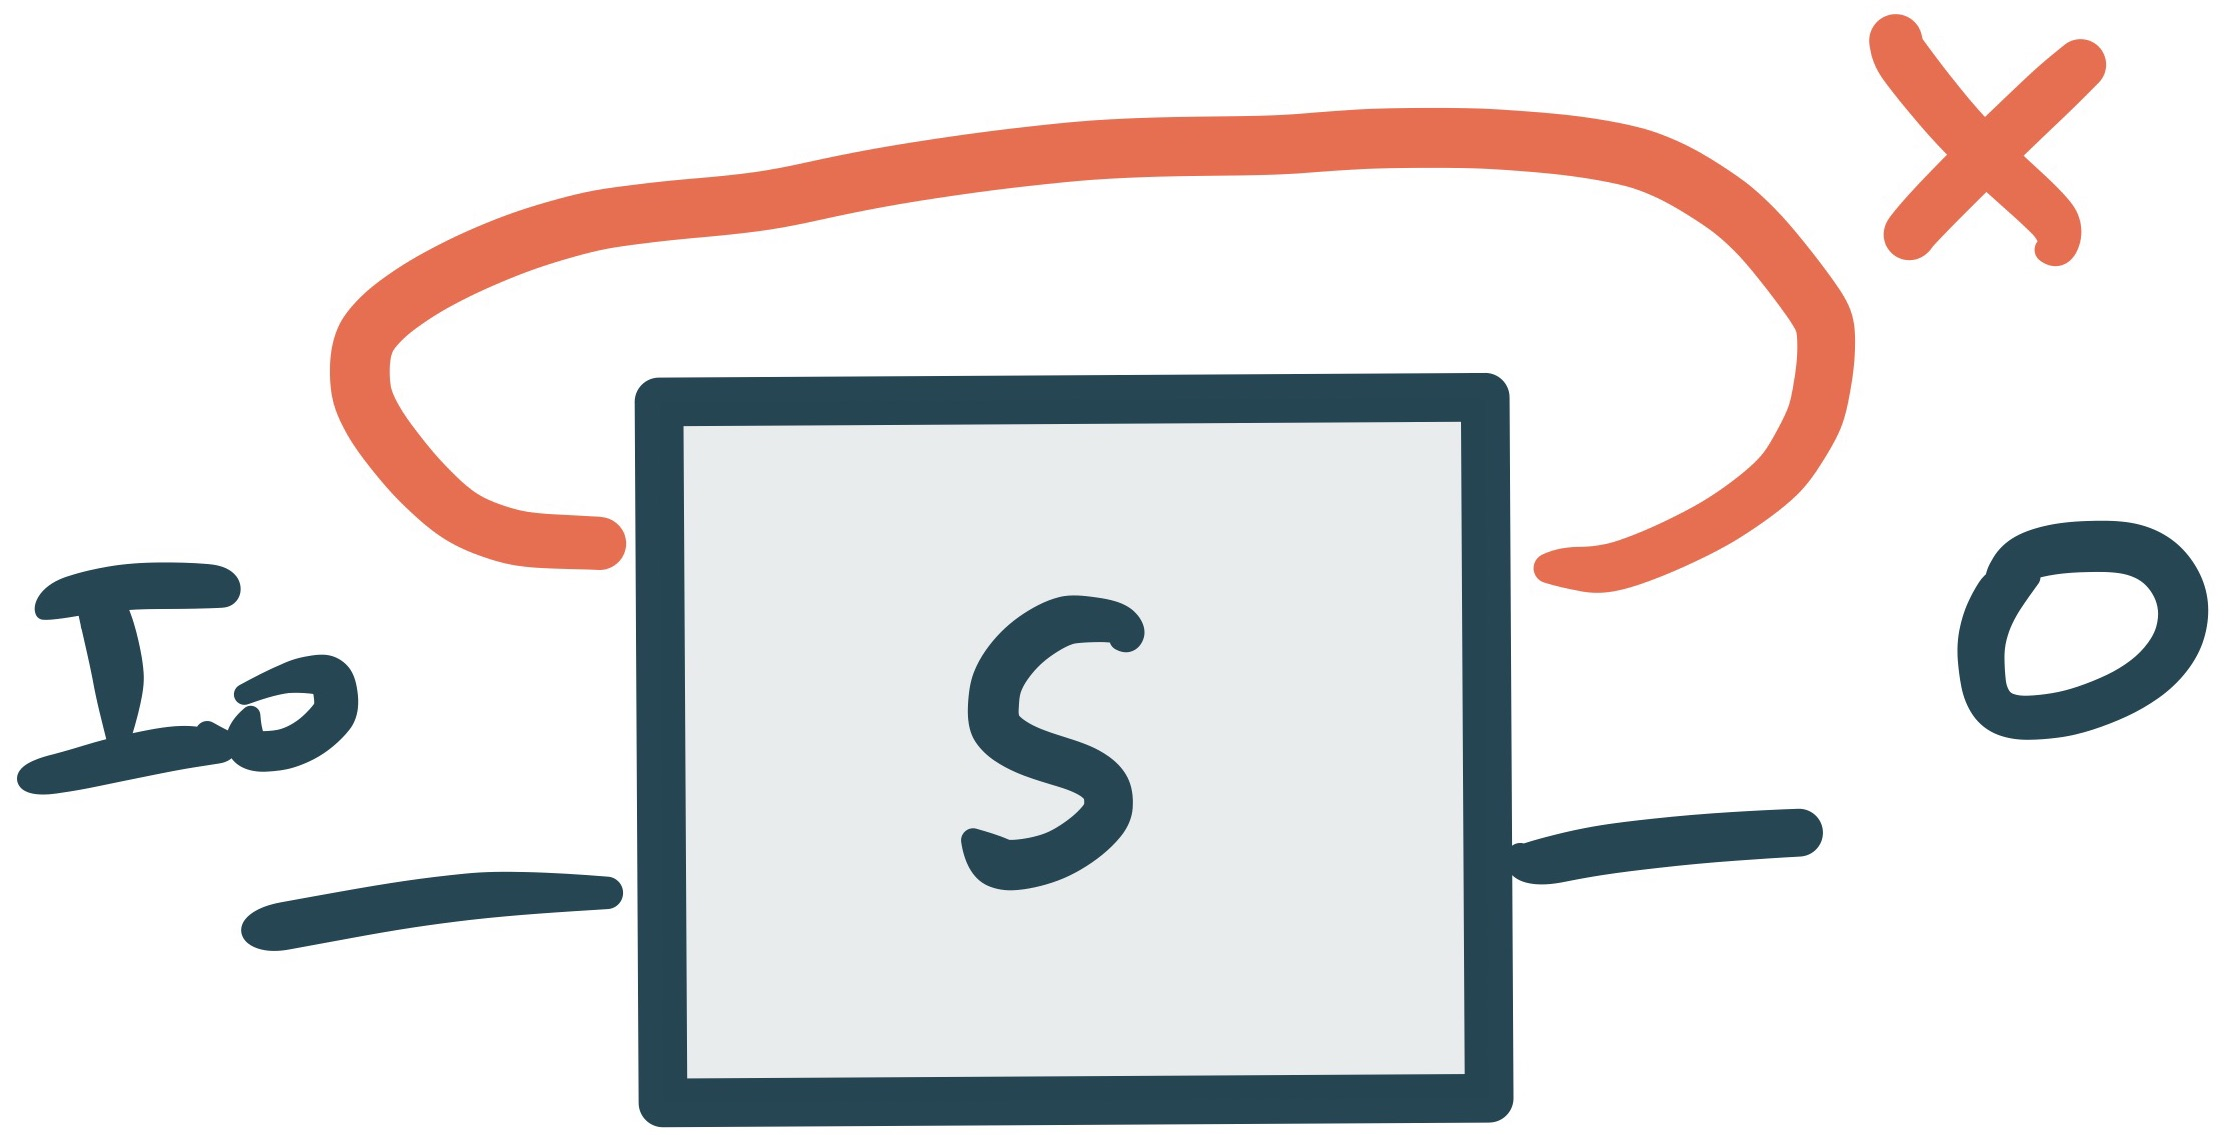
\includegraphics[width = 0.4\textwidth]{trace.jpg}
\end{center}
Formally this is done by composing $\mc{S}$ with an appropriate wrapper lens that does the rerouting. The effect of this operations is that the update and output functions are modified to 
$$up_\dagger(s, i) := up(s,\pi_1(out(s)),i),$$ 
$$out_\dagger(s) := \pi_2(out(s)).$$

Let's think about what happens to the steady-states of $\mc{S}$ under this operation. We claim that the entries of the steady-state matrix of $S^\dagger$ are 
$$m^{\mc{S}^\dagger}_{i,o} = \sum_{x \in X} m^{\mc{S}}_{(x,i)(x,o)}.$$
To see this, consider and $i,o$-steady-state $s$ of $\mc{S}^\dagger$. This satisfies $out_\dagger(s) = o$ and $up_\dagger(s,i) = s$. By definition $out_\dagger(s) = \pi_2(out(s))$, so $out(s) = (x,o)$ for some $x$. Moreover, $s = up_\dagger(s,i) = up(s,(\pi_1(out_s),i)) = up(s,(x,i))$, so $s$ is also an $(x,i),(x,o)$-steady-state of $\mc{S}$. Conversely, any $(x,i),(x,o)$-steady-state $s$ satisfies $out(s) = (x,o)$ and $up(s,(x,i)) = s$. Hence $out_\dagger(s) = o$ and $up_\dagger(s,i) = up(s,(\pi_1(out(s)),i)) = up(s,(x,i)) = s$. So $s$ is an $i,o$-steady-state of $\mc{S}^\dagger$. 

\subsubsection{Back to codesign}
We can now apply the above ideas to the parametrized system $\mc{P}$ representing to feasibility relation $\Phi: R \bprof F$. Recall that we wrote $\Phi = \bigcup_{i \in I} \varphi_i$ as a union of monotone functions $\varphi_i \colon R_i \rightarrow F$. Then the system takes inputs $(i, r) \in (I \times R_i)_{i \in I}$ and outputs $\varphi_i(r) \in F$. It has states $S := \{ (i,\varphi_j(r)) : i,j \in I, r \in R_j \}$, with identity on-positions map $(i,\varphi_j(r)) \mapsto (i,\varphi_j(r))$, and on-directions map $(i,\varphi_j(x))\mapsto (k,r \in R_i) \mapsto (k,\varphi_i(r))$.

Observe that an $(i,r),(j,f)$-steady-state of $\mc{P}$ is $s = (k,\varphi_l(r))$ satisfying $(j,f) = out(s) = (k,\varphi_l(r))$ and $s = up(s,(i,r)) = (i,\varphi_k(r))$. Hence $i=j=k$ and $f = \varphi_i(r)$. Therefore
$$M_\mc{P}(i,r)(j,f) = \begin{cases} (i,\varphi_i(r)), & \text{if } i=j \text{ and } \varphi_i(r) = f, \\ \emptyset, & \text{else.} \end{cases} $$

We now plug the output parameter $i \in I$ back as input into the system to get $\mc{P}^\dagger$:
\begin{center}
	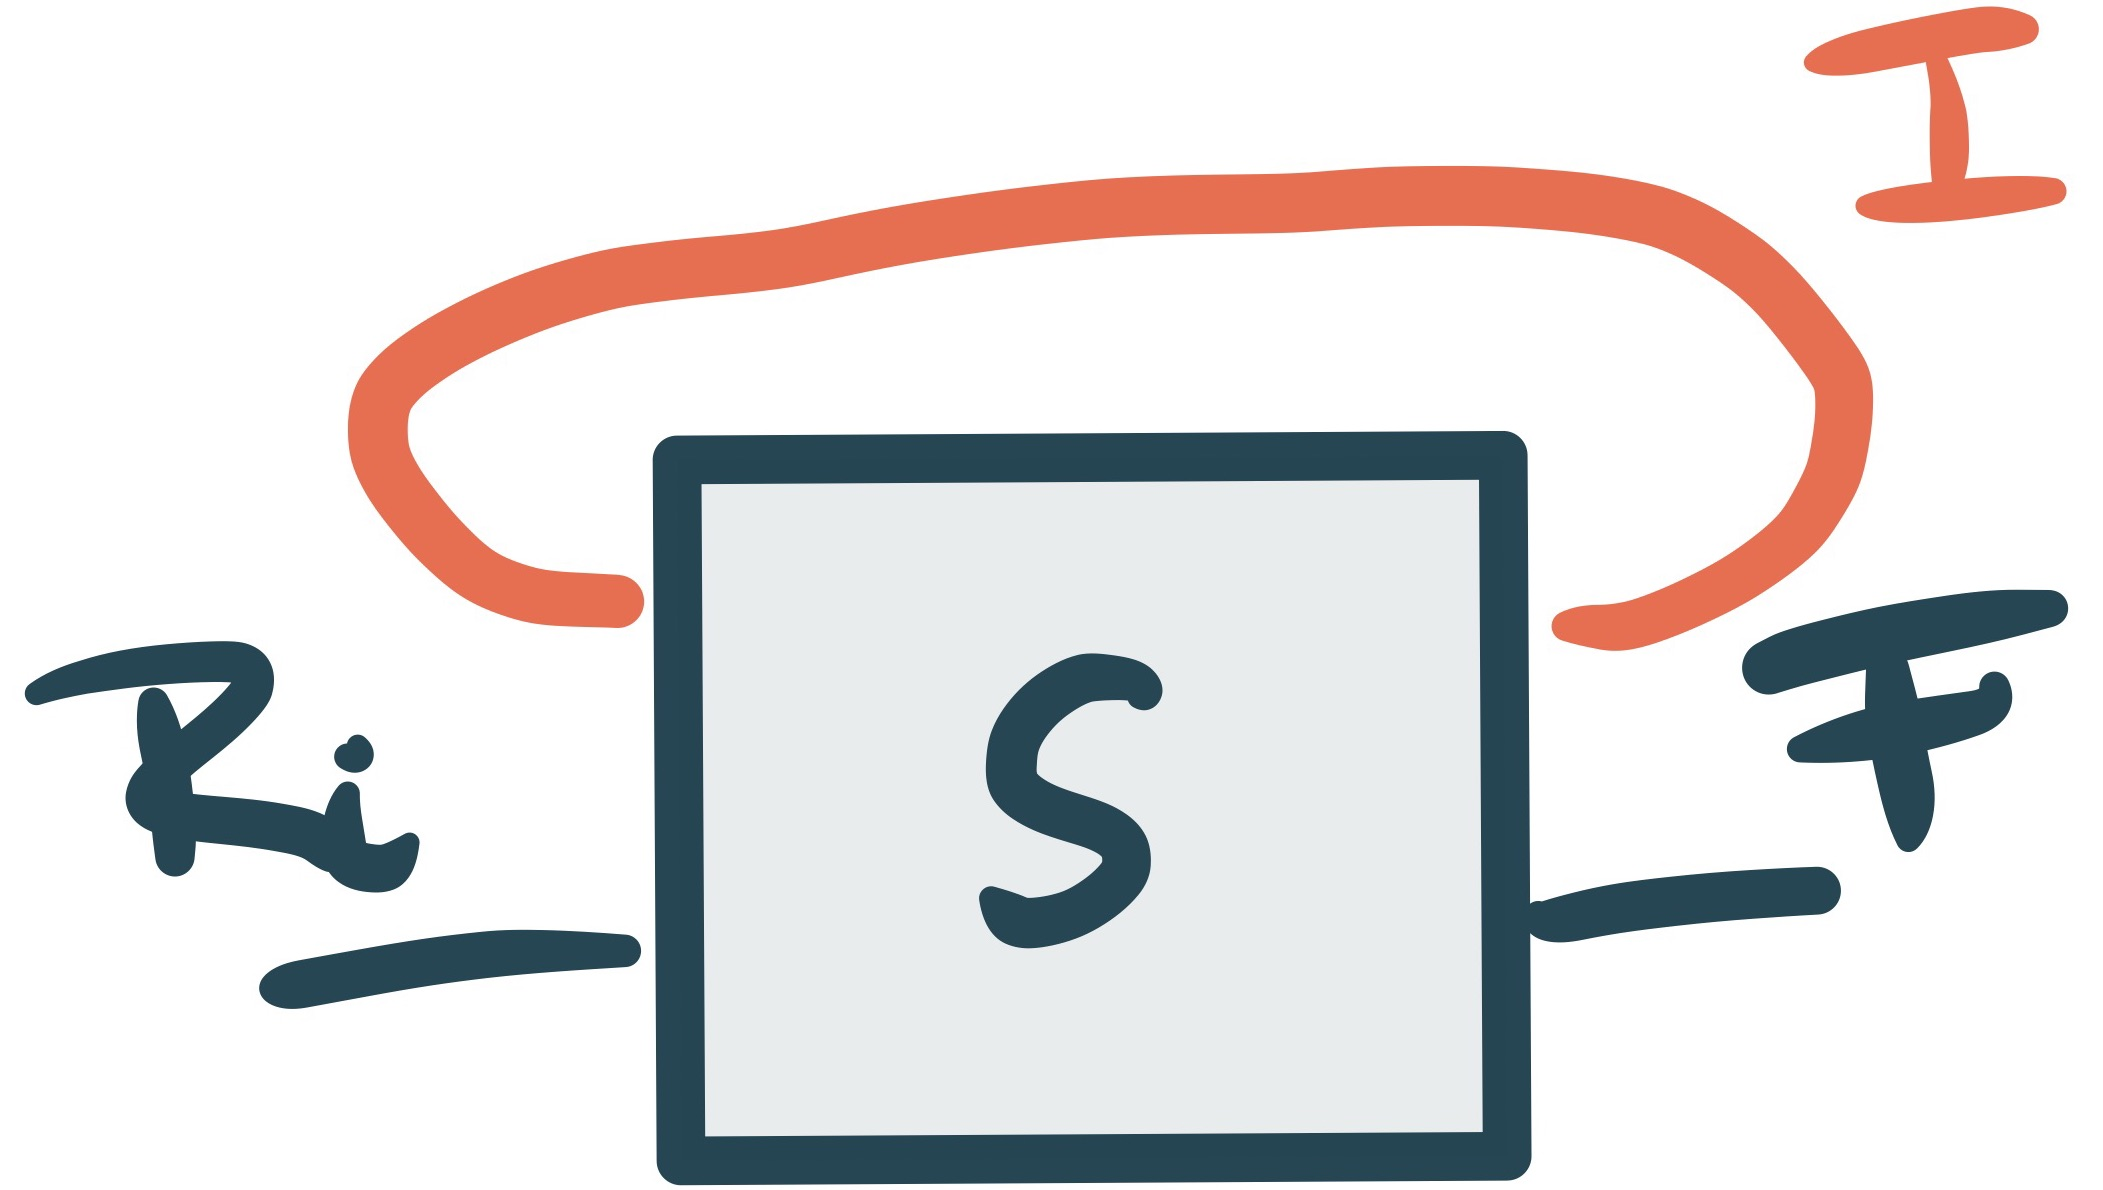
\includegraphics[width = 0.4\textwidth]{parameter-trace.jpg}
\end{center}

The steady states of $\mc{P}^\dagger$ are given by
\begin{IEEEeqnarray*}{rCl}
	m^{\mc{P}^\dagger}_{r,f} &=& \sum_{i \in I} m^\mc{P}_{(i,r)(i,f)} \\
	&=& \sum_{i \in I} \begin{cases} (i,\varphi_i(r)), & \text{if } i=i \text{ and } \varphi_i(r) = f, \\ \emptyset, & \text{else.} \end{cases} \\
	&=& \{(i,\varphi_i(r)) : \varphi_i(r) = f\}.
\end{IEEEeqnarray*}
Hence $m^{\mc{P}^\dagger}_{r,f}$ is non-empty iff $\varphi_i(r) = f$ for some $i$ iff $\Phi(r,f)$ is feasible. So the steady-state matrix $M_{\mc{P}^\dagger}$ is essentially just the matrix associated to the relation $\Phi$ (although the matrix could contain sets with multiple elements if our decomposition of $\Phi$ was not disjoint). We will interpret $m^{\mc{P}^\dagger}_{r,f}$ as the set of ways to transform $r$ into $f$. Hence we have shown that we can encode a feasibility relation $\Phi$ into a system $\mc{P}^\dagger$ whose steady states are precisely the transformations of $\Phi$.

\subsubsection{Compatibility with composition and other operations}
Now let $\mc{P}$ be a system representing $\Phi: R \prof F$ and $\mc{Q}$ be a system representing $\Psi: F \prof G$ (in the sense that the entries of the steady state matrix of the system in question has the same cardinality as the matrix representing the feasibility relation). The matrix of steady-states of the sequential composite can be calculated by $M_{\mc{P} \triangleleft \mc{Q}} = M_{\mc{P}} \cdot M_\mc{Q}$ where $(M_{\mc{P}} \cdot M_\mc{Q})_{r,g} = \sum_{f \in F} m^{\mc{P}}_{r,f} \times m^\mc{Q}_{f,g}$. On the other hand, $\Psi \circ \Phi (r,g) = \bigvee_{f \in F} \Phi(r,f) \wedge \Psi(f,g)$. So the sequential composite $\mc{P} \triangleleft \mc{Q}$ has almost the same steady-states as a system representing $\Psi \circ \Phi$. The only difference is that the sequential composition of systems also keeps track of the possible ways on can transform $r$ into $g$. The above compatibility kind of looks like a functoriality condition, but keep in mind that the sequential product $\triangleleft$ is not the default composition operation in the category of mode-dependent lenses.

We also have compatibility with the parallel product: If $\mc{P}$ represents $\Phi: R \prof F$ and $\mc{Q}$ represents $\Psi: R' \prof F'$, then the steady-states of the parallel product $\mc{P} \otimes \mc{Q}$ are given by $m^{P \otimes Q}_{(r,r'),(f,f')} = m^P_{r,f} \times m^Q_{r',f'}$. On the other hand, $\Phi \otimes \Psi ((r,r'),(f,f')) = \Phi(r,f) \wedge \Psi(r',f')$. This shows that $M_{P \otimes Q}$ is the same as the steady-state matrix of a system representing $\Phi \otimes \Psi$.

\begin{question}
	What system has the disjoint union of the steady states of its components? This would amount to taking the direct sum of the steady-state matrices.
\end{question}

Answer: Let $\mc{S} := \lens{up_S}{out_S} \colon \lens{(S)_{s \in S}}{S} \leftrightarrows \lens{(I_o)_{o \in O}}{O}$ and $\mc{T} := \lens{up_T}{out_T} \colon \lens{(T)_{t \in T}}{T} \leftrightarrows \lens{(J_u)_{u \in U}}{U}$. Define 
$$\mc{S} \sqcup \mc{T} \colon \lens{(S \sqcup T)_{x \in S \sqcup T}}{S \sqcup T} \leftrightarrows \lens{(L_y)_{y \in O \sqcup U}}{O \sqcup U}$$ 
where 
$$L_y = \begin{cases} I_y & y \in O \\ J_y & y \in U. \end{cases}$$
with on-positions function 
$$x \mapsto \begin{cases} out_S(x) & x \in S \\ out_T(x) & x \in T. \end{cases}$$ 
and on-directions function 
$$ x \mapsto \begin{cases} i \in I_x \mapsto up_S(x,i) & x \in S \\ j \in J_x \mapsto up_T(x,j) & x \in T. \end{cases}$$
The steady-state matrix of this system will satisfy 
$$m^{S \sqcup T}_{x,y} = \begin{cases} m^S_{x,y} & y \in O, x \in I_o \\  m^T_{x,y} & y \in U, x \in J_u \\ \emptyset & \text{else.} \end{cases} = (M_S \oplus M_T)_{x,y}.$$

\begin{question}
	Think about how linear algebra concepts translate: Hadamard product, inverses, spectral theorem, inner products, orthogonal matrices, norms, ect. How much of linear algebra translates to matrices valued in a monoid like $\mathbb{N}$?
\end{question}

\subsection{Introducing dynamics}
In the previous section, our machine always had the same set of modes available at any time. We will now allow the available modes of the machine to change according to its operating history. To analyze the capabilities of such a machine we will now look at trajectories rather than steady-states.

\subsubsection{Dependency graphs}
The available modes a machine has will be encoded in its dependency graph:
\begin{tcdefinition}{Dependency graph}{dependency-graph}
	A \emph{dependency graph} it a labeled directed hierarchical graph. It consists of a collection $\mc{N} := (M_t)_{t \in T}$ where each $M_t := \{ m_{t,i} : i \in I_t\}$ is a collection of modes, and for all $t \in T$ and $i \in I_t$ there is a labeled set of directed edges going from $m_{t,i}$ to elements of $\mc{N}$. The directed edges labels have the form $(r \leadsto f)$, where $r$ is a resource, and $f$ a functionality. Moreover, for each $m_{t,i}$ there is at most one edge with resource component $r$, that is we can't simultaneously have edges $(r \leadsto f)$ and $(r \leadsto g)$.
	
	The set $M_t$ expresses the modes that the machine has available at time $t$. If we select one of those modes $m_{i,t}$, the edges emanating from $m_{i,t}$ express the different options of resources we can input into the machine when it is running in mode $m_{i,t}$. If we choose a valid input $r$, we follow the edge labeled $(r \leadsto f)$ to a new set of modes $M_{t'}$ that become available in the next time-step. During this transition the machine will output $f$.
\end{tcdefinition}

\begin{tcexample}{}{}

\end{tcexample}

\begin{tcremark}{Dependency Graph as Mealy machine}{dep-mealy}
	The dependency graph is essentially a compact representation of a type of Mealy machine. To convert the dependency graph into a Mealy machine, view each edge $m_{t,i} \rightarrow M_{t'}$ labeled by $(r \leadsto f)$ as a set of edges $m_{t,i} \rightarrow m_{t',j}$ labeled by $((j,r) \leadsto f)$ for all $j \in I_{t'}$. In the dependency graph we are simply conceptually separating the inputting of resources from the choice of mode which is possible since all combinations are allowed. Finally, the mode-dependent system corresponding to a dependency graph will simply be the mode-dependent system associated to the Mealy machine obtained in this way.
\end{tcremark}

\begin{tcexample}{Converting dependency graph to dependent relations}{}
	Given a dependency graph, we can recover a relation $\mc{M}_t$ for each collection of modes $M_t$ by setting $\mc{M}_t(r,f) = \mathtt{true}$ iff there exists a $m_{t,i}$ with outgoing edge $(r \leadsto f)$. We can now assemble these relations $\mc{M}_t$ into a new labeled directed graph with nodes $\{\mc{M}_t : t \in T\}$ by contracting each set of nodes $M_t$ to a single node $\mc{M}_t$ while preserving the directed edges and their labels. More precisely, we put a
	labeled directed edge $(r \leadsto f) \colon \mc{M}_t \rightarrow \mc{M}_{t'}$ iff there exists $m_{t,i} \in M_t$ with an edge $(r \leadsto f) \colon m_{t,i} \rightarrow M_{t'}$ for some $t' \in T$. We will call this new directed labeled graph a \emph{dependent relation}.
	
	Suppose we fix an ordering on the resources and functionalities appearing in the edge labels. Then the $\mc{M}_t$ are relations between preorders. If all relations $\mc{M}_t$ are feasibility relations, we will call the dependency graph \emph{monotone}. Each $M_t$ in a monotone dependency graph will satisfy:
	\begin{itemize}
		\item[(i)] If $r \leq s$ and there is an edge $(r \leadsto f) \colon m_{t,i} \rightarrow M_{t'}$, then there is also an edge $(s \leadsto f) \colon m_{t,i'} \rightarrow M_{t''}$, 
		\item[(ii)] If $f \leq g$ and there is an edge $(r \leadsto g) \colon m_{t,i} \rightarrow M_{t'}$, then there is also an edge $(r \leadsto f) \colon m_{t,i'} \rightarrow M_{t''}$.
	\end{itemize}
	Conversely, any monotone dependency graph gives rise to a dependent relation whose nodes are all feasibility relations.
\end{tcexample}

\begin{tcexample}{Converting dependent feasibility relations to monotone dependency graph}{}
	Suppose we are given a dependent relation whose nodes are all feasibility relations. Explicitly, we consider a collection of feasibility relations $\Phi_t \colon R_t \rightarrow F_t$. A dependent feasibility relation with nodes $\Phi_t$ is a labeled directed graph where for each node $\Phi_t$ we have outgoing directed edges labeled by $(r \leadsto f)$ for each feasible pair $(r,f) \in \Phi_t$.

	We can convert such a dependent feasibility relation to a monotone dependency graph by choosing a mode decomposition $\Phi_t = \bigcup_{i \in I_t} \varphi_{t,i}$ for each $t \in T$, where the $\varphi_{t,i} \colon: R_{t,i} \rightarrow F_t$ are monotone maps. We then set $M_t := \{ \varphi_{t,i} : i \in I_t \}$ and for each $\varphi_{t,i}$ we put an outgoing labeled edge $(r \leadsto f) \colon : \varphi_{t,i} \rightarrow M_{t'}$ iff $\varphi(r) = f$ and there is a labeled edge $(r \leadsto f) \colon \Phi_t \rightarrow \Phi_t'$ in the dependent feasibility relation. In other words, we are expanding each node $\Phi_t$ to a set of modes and partitioning the labeled edges accordingly.
\end{tcexample}

Given a dependency graph we can construct a mode-dependent system associated to it in the following way:
\begin{tcdefinition}{System associated to dependency graph}{}
	Let $\mc{G}$ be a dependency graph with nodes $(M_t)_{t \in T}$ where $M_t  = (m_{t,i})$ for $i \in I_t$. If $m_{t,i} \in M_t$ is a mode, then denote by $\mathsf{edge}(m_{t,i})$ the set of labels of edges emanating from $m_{t,i}$. Denote further $R_{t,i} := \{ r : (r \leadsto f) \in \mathsf{edge}(m_{t,i}) \text{ for some } f\}$ and $F_{t,i} := \{ f : (r \leadsto f) \in \mathsf{edge}(m_{t,i}) \text{ for some } r\}$. Let $F := \bigcup_{t \in T, i \in I_t} F_{t,i}$ and $I := \bigsqcup_{t \in T} I_t$. For each $m_{t,i}$ we define a function $\mathsf{succ}_{t,i} \colon R_{t,i} \times T \rightarrow T$ which sends $(r,t) \mapsto t'$ where $t'$ is the index of the target of the unique emanating edge $(r \leadsto f) \colon m_{t,i} \rightarrow M_{t'}$. Finally, define the function $\mathsf{return}_{t,i} \colon R_{t,i} \rightarrow F_{t,i}$ which sends $r$ to the unique functionality $f$ for which there is an emanating edge $(r \leadsto f) \colon m_{t,i} \rightarrow M_{t'}$.
	
	We construct a system $\mathsf{Sys}(\mc{G}) \colon \lens{(S)_{s \in S}}{S} \leftrightarrows \lens{(R_{t,i})_{t \in T, i \in I_t}}{T \times I \times F}$ associated to $\mc{G}$ as follows:
	The states of $\mathsf{Sys}(\mc{G})$ are given by 
	$$S := \{ (t,i,f) : t \in T, i \in I_t, \exists (r \leadsto f) \in \mathsf{edge}(m_{t,i}) \text{ for some } r \}$$
	The output map is given by $(t,i,f) \mapsto (t,i,f)$.
	The update map is given by $ (t,i,f) \mapsto (j,r \in R_{t,i}) \mapsto (\mathsf{succ}_{t,i}(r,t),j, \mathsf{return}_{t,i}(r))$.

	Observe that this mapping is injective on isomorphisms classes of dependency graphs: We can recover the nodes $M_t = (m_{t,i})$ from the states (up to isomorphism) and recover the emanating edges from $m_{t,i}$ using the update function. If the system is in state $(t,i,f)$ (as can be seen from its output) and $up(j,r \in R_{t,i}) = (t', j, g)$, we need to put an edge $(r \leadsto g) \colon m_{t,i} \rightarrow M_{t'}$.
\end{tcdefinition}

\begin{question}
	Given two different monotone dependency graphs obtained from a given dependent feasibility relation, what is the relationship between the systems associated to each one? Will the mode-traced out systems be equivalent in the sense of bisimulation?
\end{question}

\subsubsection{Path analysis in dependency graphs}
Given a (monotone) dependency graph, we can start asking codesign-style questions:
\begin{itemize}
	\item[(a)] Given that I can provide a sequence of resources $(r_1,r_2, \ldots, r_n)$ is it possible to obtain a given sequence of functionalities $(f_1, f_2, \ldots, f_n)$?
	\item[(b)] Given that I can provide a sequence of resources $(r_1,r_2, \ldots, r_n)$ is it possible to obtain a specific functionality $f$ at some given time?
	\item[(c)] Given that I can provide a sequence of resources $(r_1,r_2, \ldots, r_n)$ is it possible to obtain a specific functionality $f$ at some time (don't care when)?
	\item[(d)] If I want to get functionality $f$ at time $t$, what is the cheapest sequence of resources $(r_1,r_2, \ldots, r_n)$ that will achieve this? 
	\item[(e)] If I want to get a specific sequence of functionalities $(f_1, f_2, \ldots, f_n)$, what is the cheapest sequence of resources $(r_1,r_2, \ldots, r_n)$ that will achieve this?
\end{itemize}

Notice that all these questions can be phrased using sequences of resources and functionalities. The question (a) asks whether there is a path through the dependency graph labeled by $(r_1 \leadsto f_1), \ldots, (r_n \leadsto f_n)$. The questions (b) and (c) can be reduced to this question by considering a larger class of desirable output sequences. Questions (d) and (e) additionally involve the notion of minimization. For this we need to order sequences of resources by their value.

\begin{tcdefinition}{Feasibility on sequences}{feas-seq}
	Let $\mc{G}$ be a dependency graph and let $\mathbf{r} := (r_1,\ldots,r_n)$ be a sequence of resources and $\mathbf{f} := (f_1, \ldots, f_n)$ be a sequence of functionalities. The pair $(\mathbf{r},\mathbf{f})$ is feasible iff there exists a path $(r_1 \leadsto f_1), \ldots, (r_n \leadsto f_n)$ in $\mc{G}$.
\end{tcdefinition}

\begin{tctheorem}{}{}
If $\mc{G}$ is a monotone dependency graph which was obtained from a dependent feasibility relation $(\Phi_t \colon R_t \bprof F_t)_{t \in T}$, then $(\mathbf{r},\mathbf{f})$ is feasible iff
\begin{itemize}
	\item[(i)] $(r_i, f_i) \in \Phi_{t_i}$ for all $1 \leq i \leq n$,
	\item[(ii)] $\Phi_{t_{i+1}} = \Phi_{\mathsf{next}_{t_i}(r_i, f_i)}$ for all $t_i$,
\end{itemize}
where $\mathsf{next}_t : R_t \times F_t \rightarrow T$ maps $(r, f) \mapsto t'$ where $t'$ is the index associated with the target of the unique edge $(r \leadsto f) \colon \Phi_i \rightarrow \Phi_{t'}$.
\end{tctheorem}

\begin{tcdefinition}{Regular dependent feasibility relation}{}
	\begin{itemize}
		\item[(i)] $r \leq s$ and $(r \leadsto f) \colon \Phi_i \rightarrow \Phi_j$ implies $(s \leadsto f) \colon \Phi_i \rightarrow \Phi_j$,
		\item[(ii)] $f \leq g$ and $(r \leadsto g) \colon \Phi_i \rightarrow \Phi_j$ implies $(r \leadsto f) \colon \Phi_i \rightarrow \Phi_j$.
	\end{itemize}
\end{tcdefinition}

\begin{tctheorem}{}{}
	For a regular dependent feasibility relation, feasibility of sequences is a feasibility relation $\Theta \colon R^n \bprof F^n$ when considering the product ordering on $R = \bigcup_t R_t$ and $F = \bigcup_t F_t$.
\end{tctheorem}

\subsubsection{Valuating sequences of resources}

\subsubsection{Algorithmic aspects}
If we care about the product ordering on sequences, it seems like we could find minimal paths (in terms of resource cost) by optimizing at each step, i.e taking the edge with our desired functionality that has minimal cost.


\subsubsection{Trajectory analysis}
If we think about the system associated to a dependency graph, path analysis becomes trajectory analysis. The systems picture is particularly useful if we want to think about composing systems by wiring them together.

\begin{tcdefinition}{Trajectories}{trajectories}
	Let $\mc{S} := \lens{up_S}{out_S} \colon \lens{(S)_{s \in S}}{S} \leftrightarrows \lens{(I_o)_{o \in O}}{O}$ and consider the system $\mc{T} \colon \lens{(\mathbb{N})_{n \in \mathbb{N}}}{\mathbb{N}} \leftrightarrows \lens{*}{\mathbb{N}}$ whose on-positions map is the identity and whose on-directions map sends $n \mapsto * \mapsto n+1$.

	A chart $\lens{f_\flat}{f} \colon \lens{*}{\mathbb{N}} \rightrightarrows \lens{(I_o)_{o \in O}}{O}$ consists of a sequence $f \colon \mathbb{N} \rightarrow O$ and a dependent function $f_\flat \colon (n \in \mathbb{N}) \rightarrow * \rightarrow I_{f(n)}$. We can identify the latter with a sequence $(a_0, a_1, \ldots)$ where each $a_i \in I_{f(i)}$.

	Given sequences $o \in \prod_{n \in \mathbb{N}} O$ and $i \in \prod_{n \in \mathbb{N}} I_{o(n)}$, an $i,o$-trajectory in $\mc{S}$ consists of a sequence $s \colon \mathbb{N} \rightarrow S$ such that for all $n \in \mathbb{N}$ we have
	$$out(s(n)) = o(n), $$
	$$s(n+1) = up(s(n), i(n)).$$
\end{tcdefinition}

\begin{question}
	Go through all composition operations for systems associated to dependency graphs and see if they translate back to natural operations on dependency graphs.
\end{question}

\end{document}